\documentclass{standalone}
\usepackage{graphicx}	
\usepackage{amssymb, amsmath}
\usepackage{color}

\usepackage{tikz}
\usetikzlibrary{intersections, backgrounds, math}
\usepackage{pgfmath}

\definecolor{light}{RGB}{220, 188, 188}
\definecolor{mid}{RGB}{185, 124, 124}
\definecolor{dark}{RGB}{143, 39, 39}
\definecolor{darker}{RGB}{124, 0, 0}
\definecolor{highlight}{RGB}{180, 31, 180}
\definecolor{light_teal}{RGB}{107, 142, 142}
\definecolor{mid_teal}{RGB}{72, 117, 117}
\definecolor{dark_teal}{RGB}{29, 79, 79}
\definecolor{gray10}{gray}{0.1}
\definecolor{gray20}{gray}{0.2}
\definecolor{gray30}{gray}{0.3}
\definecolor{gray40}{gray}{0.4}
\definecolor{gray60}{gray}{0.6}
\definecolor{gray70}{gray}{0.7}
\definecolor{gray80}{gray}{0.8}
\definecolor{gray90}{gray}{0.9}
\definecolor{gray95}{gray}{0.95}

\begin{document}

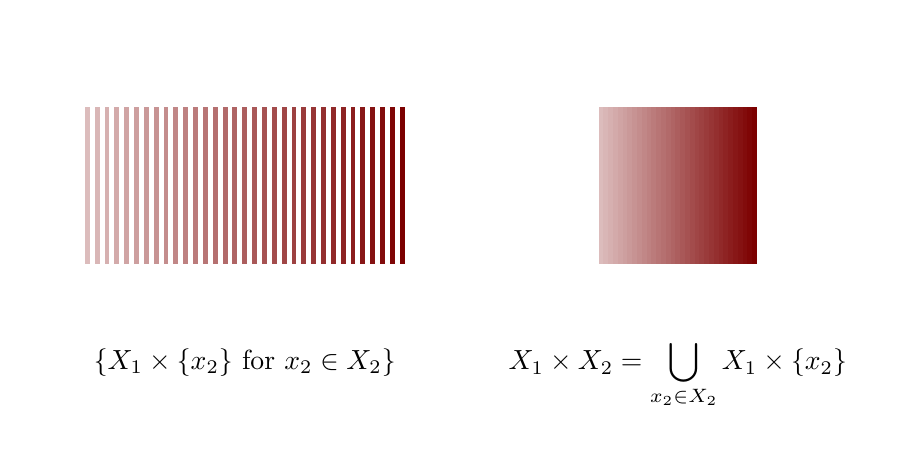
\begin{tikzpicture}[scale=1.0]
 
  \pgfmathsetmacro{\delta}{1 / 32}
  
  \draw[white] (-2.75, -3) rectangle (2.75, 2);
  
  \foreach \n in {0, 1, ..., 32} {
    \pgfmathsetmacro{\xi}{2 * (\n / 16 - 1)}
    \pgfmathsetmacro{\prop}{100 * \n / 32}
    \colorlet{custom}{darker!\prop!light};
    \fill[custom]    (\xi - \delta, -1) -- (\xi + \delta, -1) 
                  -- (\xi + \delta, 1) -- (\xi - \delta, 1) -- cycle;
  }
      
  \node at (0, -2.25) { $ \{ X_{1} \times \{ x_{2}  \} \text{ for } x_{2} \in X_{2} \}$ };
  
  \begin{scope}[shift={(5.5, 0)}]
  
  \draw[white] (-2.75, -3) rectangle (2.75, 2);
  
  \foreach \n in {0, 1, ..., 32} {
    \pgfmathsetmacro{\xi}{0.975 * (\n / 16 - 1)}
    \pgfmathsetmacro{\prop}{100 * \n / 32}
    \colorlet{custom}{darker!\prop!light};
    \fill[custom]    (\xi - \delta, -1) -- (\xi + \delta, -1) 
                  -- (\xi + \delta, 1) -- (\xi - \delta, 1) -- cycle;
  }
      
  \node at (0, -2.4) 
    { $X_{1} \times X_{2} = \displaystyle \bigcup_{x_{2} \in X_{2}} X_{1} \times \{ x_{2}  \}$ };
  
  \end{scope}

\end{tikzpicture}

\end{document}  